\section{Sorting algorithms}

In this section I will revisit the four sorting algorithms that are a must-know for coding interviews.
I will start with some basic considerations on what to look for on a sorting algorithm and why there is not a \emph{perfect} sorting algorithm.
After that, I visit the four most commonly used in coding interviews.
For each of them, I will show the general algorithm in pseudocode and then two implementations:
\begin{enumerate}
 \item An implementation using arrays of integers since this is the easiest to understand.
 \item An implementation using the \href{https://en.wikibooks.org/wiki/More_C\%2B\%2B_Idioms/Iterator_Pair}{iterator idiom} in C++. Since this is the trickiest, and therefore asked in many interview questions.
\end{enumerate}

\subsection{Desired properties for sorting algorithms}

The sorting problem states that: Given a \emph{collection} (very likely and array) of $n$ \emph{elements} (usually assumed to be numbers, without loss of generality) and an \emph{order} defined on the elements (a way of telling for each two of them who is the lesser or if they are equal), we are interested in an algorithms that is able to return a permutation $(e_1, e_2, \ldots, e_n)$ of the elements in the collection such that $e_i \leq e_{i + 1}$, for $i \in [1, n-1]$

It is shown in any Computer Science class on Algorithms that theoretically the best running time we can achieve for a sorting algorithm is $O(n \cdot \lg n)$.

This is true only when we have \emph{certain} considerations for the computation model and the input. The most important are:

\begin{itemize}
 \item That we do not impose any restrictions on the input data. Particularly, we do not assume that the input entries are in any specific range. Nor that they are arriving at a certain time.
 \item That the algorithm is based on comparisons. In other words: the computer is only able to take \emph{two} elements at a time, from the input to compare them.
\end{itemize}

Assuming, that we have the two condition above, we are interested on an algorithm that is able to to sort the input data. 
The algorithms can have many desired properties, but the ones that we are usually interested are:

\begin{description}
 \item[Optimal] The algoritm runs in $O(n \cdot \lg n)$, for all valid inputs.
 \item[In place] The algorithm only requieres a constant $O(1)$ amount of extra space to operate.
 \item[Stable] If some elements of the input are equall, in the output those elements appear on the same order as they were in the input.
\end{description}

There has not been discover a \emph{simple} algorithm that has all these properties\footnote{Algorithms that have all these properites indeed exist. See for example \href{https://en.wikipedia.org/wiki/Block_sort}{block sort}. But they are very complex and no one will be expected to know them in a normal coding interiview}.
However, we have in particular four algorithms that have some of this properites, we can see a summary in Table~\ref{tab:sorting}.

\begin{table}[htb]
  \begin{center}
    \begin{tabular}{l | r r r | l}
      Algorithm & Optimal & In place & Stable & Comment\\
      \midrule
      Selection sort & No & Yes & No & Always runs in $O(n^2)$, but it's very easy to implement\\
      Quicksort & No & Yes & No & On average runs in $O(n \cdot \lg n)$. The worst case it's $O(n^2)$ \\
      Mergesort & Yes & No & Yes & It requieres $O(n)$ extra memory\\
      Heapsort & Yes & Yes & No & \\
    \end{tabular}
  \end{center}
\caption{Summary of the properities of the exposed algorithms}
\label{tab:sorting}
\end{table}

\subsection{Selection sort}

This is one of the simplest algorithms for sorting that exist.
If a novice programmer that has never taken a class on algorithms is asked to create a sorting algorithm, chances are that it will come up with selection sort.
The value for a coding interview is like some sort of \emph{panic sort}.

If you are tasked to create an algorithm that at some point requires sorting; and your interviewer asks you to implement to the smallest detail (which is very unlikely to happen).
You can always default back to insertion sort if you do not want to spend precious time thinking on the sorting part.
That is after saying to your interviewer that you know this is a bad algorithm, and you are using it \emph{only} because you do not have more time.

Having said that, if you face a problem where sorting is an essential part of the answer, using selection sort is a \emph{very bad} solution.

In essence, selection sort uses one simple fact:

The best way to find the minimum (or maximum for that matters) element of an array, takes $O(n)$ and it is the following:
\begin{enumerate}
 \item Assume that the minimum is the first element of the array.
 \item Compare the next element to the minimum. If that element is smaller, mark it as the new minimum.
 \item Continue doing the previous step until you reach the end of the array.
\end{enumerate}

Now that we know this simple fact, selection sort is very simple.

\begin{enumerate}
 \item Find the minimum element of the array.
 \item If the minimum is not at the beginning of the array, swap the minimum with the first element of the array.
 \item Assume that you have now a smaller array consisting of the second element of the array until the end.
 \item Repeat from step 1 until you don't have any more elements.
\end{enumerate}

Indeed selection sort have this name because at each step you \emph{select} the minimun element to place it at his corresponding place.

The Algorithm~\ref{alg:selectionsort} shows the formal details to implement selection sort.
To make the pseudocode easier I assume a zero based indexing.
In other words the first element of the array $V$ is $v_0$ and the last element is $v_{n-1}$

\begin{algorithm}[H]
\caption{Selection sort}
\label{alg:selectionsort}
\begin{algorithmic}[1] % El número le dice al entorno desde que número empezar a contar. Si le pones 0 omite los números
\Require $V = \{ v_0, v_1, \ldots, v_{n-1} \} $ \Comment{An array $V$ of size $n$}
\Ensure $V\text{ such that } v_i \leq v_{i + 1}, \forall i \in [0, n-2]$ \Comment{The array $V$ with his elements sorted}
\Procedure{InsertionSort}{$V$}
\For{$j \gets 0 \textbf{ to } n-1 \textbf{ step } 1$}
    \State $\text{min} \gets j$ \Comment{Assume the minimum is at the start}
    \For{$i \gets j+1 \textbf{ to } n-1 \textbf{ step } 1$} \Comment{Search for the actual minimum in the remainder of the interval}
        \If {$v_i < v_{\text{min}}$}
            \State $\text{min} \gets i$
        \EndIf
    \EndFor
    \If {$\text{min} \neq j$} \Comment{If the minimum it's not at the start}
        \State $\text{min} \leftrightarrow j$ \Comment{swap the two elements}
    \EndIf
\EndFor
\EndProcedure
\end{algorithmic}
\end{algorithm}

The Listing~\ref{lst:selectionsort} shows the implementation on actual C++ code using arrays. Or \mintinline{cpp}{std::vector}s to be more precise.
To be complete the Listing~\ref{lst:selectionsort} also shows an implementation of   insertion sort in C++ using iterators.

\begin{listing}
\inputminted[
  firstline=7, %If you omit this two fields, the whole file is pulled
  lastline=23
  ]{cpp}{src/sortAlgorithms.cpp}
  \caption{An implementation of insertion sort in C++ using a vector}\label{lst:selectionsort}
\end{listing}

\begin{listing}
\inputminted[
  firstline=42, %If you omit this two fields, the whole file is pulled
  lastline=59
  ]{cpp}{src/sortAlgorithms.h}
  \caption{An implementation of insertion sort in C++ using iterators}\label{lst:selectionsortiter}
\end{listing}
 
\subsection{Quicksort}

This algorithm is one of the most used algorithms in the world.
To be more precise \emph{quicksort} is a family of algorithms.
The base idea remains the same in all of them.
However, the way different algorithms of the family made the so-called \emph{partition} changes.
Such change in the partition has implications on the running time.

The two most dominant schemes of partition are Lobuto and Ohare.
Since we are studying for an interview, we are going to be using Lobuto, since the code is cleaner.
That being said, Ohare's scheme is considered a more efficient algorithm.

First we present the basic idea behind all quicksort families. 
These are divide and conquer algorithms, so they subdivide the problem and call themselves recursivelly.

\begin{enumerate}
 \item If the array to be sorted has less than 2 elements, it is already sorted; you do not need to do anything just return.
 \item Partition the array into two parts and a pivot. The first part contains all the elements smaller than the pivot, the second part contains all the elements greater than the pivot (elements equal to the pivot can go in either part)
 \item Then you can recursively use quicksort to order the two remaing parts.
\end{enumerate}

In this pseudocode I will use a zero based indexing again, that is the first element of the array $V$ is $v_0$ and the last element is $v_{n-1}$.
Also we will use indices to keep track of the interval of the original array we are sorting.
Those intervals are defined by two indices in the original array.

For defining the intervals, I use the begin and end convention.
On this convention the first index is the \emph{first} element of the interval, the second element is \emph{one pass the last} element of the interval.
For example the indices $i$, $j$, where $i \leq j$, define the interval $[i, j)$ whose first element is $v_i$ and last element is $v_{j-1}$

Since this is a recursive algorithm the first call to sort the whole array will need to be called with indices $0$ and $n$ for an array $V$ of $n$ elements

\begin{algorithm}[H]
\caption{Quicksort}
\label{alg:quicksort}
\begin{algorithmic}[1] % El número le dice al entorno desde que número empezar a contar. Si le pones 0 omite los números
\Require $V = \{ v_0, v_1, \ldots, v_{n-1} \} $ and $[b,e)$ \Comment{An array $V$ of size $n$, and an inerval $[b,e)$ with $0 \leq b \leq e \leq n$}
\Ensure $V\text{ such that } v_i \leq v_{i + 1}, \forall i \in [0, n-2]$ \Comment{The array $V$ with his elements sorted}
\Procedure{QuickSort}{$V$, $b$, $e$} \Comment{$b$ stands for \emph{begin} and $e$ for \emph{end}}
    \If {$(e - b) > 1$} \Comment{If the interval contains more than one element}
        \State $p \gets$ \Call{Partition}{$V$, $b$, $e$} \label{endPartition} \Comment{Make a partition of $V$ and get the partition point $p$}
        \State \Call{QuickSort}{$V$, $b$, $p$} \Comment{Order one half}
        \State \Call{QuickSort}{$V$, $p + 1$, $e$} \Comment{Order one other half}
    \EndIf
\EndProcedure
\Procedure{Partition}{$V$, $l$, $r$} \Comment{$l$ stands for \emph{left} and $r$ for \emph{right}}
\State $j \gets r - 1$ \label{pivotPlace} \Comment{$j$ stores the index of the pivot}
\State $p \gets l$ \Comment{$p$ stores the \emph{partition point}}
\For{$i \gets l \textbf{ to } j-1 \textbf{ step } 1$} \Comment{We traverse the interval minus the pivot (which it's at the end)}
    \If {$v_i \leq v_j$} \Comment{If this element is smaller than the pivot}
        \State $v_p \leftrightarrow v_i$ \Comment{swap it with the one at the partition point}
        \State $p \gets p + 1$ \Comment{Move the partition point}
    \EndIf
\EndFor
\State $v_p \leftrightarrow v_j$ \Comment{Put the pivot in his corresponding place}
\State \Return $p$ \Comment{return the partition point}
\EndProcedure
\end{algorithmic}
\end{algorithm}

A couple of remarks to clarify the above pseudocode.
\begin{itemize}
 \item After the call to \emph{partition} in line~\ref{endPartition}, the only element we can guarantee to be at his corresponding place (in the ordered array) is the pivot.
 \item In Loboto's partition scheme, we choose the last element of the interval to be the \emph{pivot} element.
 \item The variable $j$ on line~\ref{pivotPlace} it's not really needed. It just makes the code easier to read by marking the initial place of the pivot.
 \item The variable $p$ is the \emph{partition point}: the place at which the pivot will be at the end of the partition procedure.
 \item The way the scheme works is \emph{assuming} that all the elements less than the pivot are to the left of $p$. If we found some element that it is not, then we change his place and move $p$ (Since now we have another element that should be at his left).
\end{itemize}

The code using an array is strightfoward to implement and is shown in two parts: The Listing~\ref{lst:quicksortArray} shows the main quicksort function and the Listing~\ref{lst:partitionArray} shows the partition scheme (Lobuto).

\begin{listing}
\inputminted[
  firstline=52, %If you omit this two fields, the whole file is pulled
  lastline=69
  ]{cpp}{src/sortAlgorithms.cpp}
  \caption{An implementation of quicksort in C++ using an array}\label{lst:quicksortArray}
\end{listing}

\begin{listing}
\inputminted[
  firstline=25, %If you omit this two fields, the whole file is pulled
  lastline=51
  ]{cpp}{src/sortAlgorithms.cpp}
  \caption{The partition (Lobuto) used by quicksort in C++}\label{lst:partitionArray}
\end{listing}

Since we already have the range defined in a very similar way to that of an iterator. 
The code to implement both functions using C++ iterators it's very similar.
Listing~\ref{lst:quicksortIterator} shows the implementation of the main function and Listing~\ref{lst:partitionIterator} the partition scheme.

\begin{listing}
\inputminted[
  firstline=27, %If you omit this two fields, the whole file is pulled
  lastline=40
  ]{cpp}{src/sortAlgorithms.h}
  \caption{An implementation of quicksort in C++ using iterators}\label{lst:quicksortIterator}
\end{listing}

\begin{listing}
\inputminted[
  firstline=3, %If you omit this two fields, the whole file is pulled
  lastline=25
  ]{cpp}{src/sortAlgorithms.h}
  \caption{Lobuto's partition using iterators}\label{lst:partitionIterator}
\end{listing}

\subsection{Mergesort}

This is another divide and conquer algorithm.
This is also an optimal algorithm, it always runs in $O(n \cdot \lg n)$.
Mergesort is also a stable algorithm and it's somehow easy to implement.
The only drawback is that it requires an extra $O(n)$ of space to operate.
In other words this is \emph{not} an in place algorithm.

The idea behind merge sort is \emph{similar} to quicksort in the sense that first divides the input in two and then sorts recursively the resulting parts.
Therefore, it will also require to keep track of the interval $[b,e)$ that is currently sorting.

The array is first divided in halves and then each half is sorted.
Then, both (already ordered) halves are \emph{merge} into a complete sorted array.
The pseudocode for Mergesort is shown in the Algorithm~\ref{alg:mergesort}.

\begin{algorithm}[H]
\caption{Merge sort}
\label{alg:mergesort}
\begin{algorithmic}[1] % El número le dice al entorno desde que número empezar a contar. Si le pones 0 omite los números
\Require $V = \{ v_0, v_1, \ldots, v_{n-1} \} $ and $[b,e)$ \Comment{An array $V$ of size $n$, and an interval $[b,e)$ with $0 \leq b \leq e \leq n$}
\Ensure $V\text{ such that } v_i \leq v_{i + 1}, \forall i \in [0, n-2]$ \Comment{The array $V$ with his elements sorted}
\Procedure{MergeSort}{$V$, $b$, $e$} \Comment{$b$ stands for \emph{begin} and $e$ for \emph{end}}
    \If {$(e - b) > 1$} \Comment{If the interval contains more than one element}
        \State $m \gets \frac{(e + b)}{2}$ \Comment{Calculate the middle point of the array}
        \State \Call{MergeSort}{$V$, $b$, $m$} \Comment{Order one half}
        \State \Call{MergeSort}{$V$, $m$, $e$} \Comment{Order one other half}
        \State \Call{Merge}{$V$, $b$, $m$, $e$} \Comment{Merge the sorted halves to create a complete sorted array}
    \EndIf
\EndProcedure
\Procedure{Merge}{$V$, $b$, $m$, $e$} \Comment{$b$ stands for \emph{begin}, $m$ for \emph{middle} and $e$ for \emph{end}}
\State $l \gets b$  \Comment{$l$ stores the current index of the \emph{low} half}
\State $h \gets m$ \Comment{$h$ stores the current index of the \emph{high} half}
\For{$i \gets b \textbf{ to } e-1 \textbf{ step } 1$} \label{merge:loop} \Comment{Merge the two halves in a temporal buffer $B$}
    \If {$l < m \textbf{ and }(V_{l} \leq V_{h} \textbf{ or } h \geq e )$} \label{merge:condition}\Comment{See explanation below}
        \State $B_i \gets V_l$ \Comment{Take the one from the lower half}
        \State $l \gets l + 1$
    \Else
        \State $B_i \gets V_h$ \Comment{Take the one from the higher half}
        \State $h \gets h + 1$
    \EndIf
\EndFor
\State $j \gets 0$ \Comment{A variable to keep track of the place in $B$}
\For{$i \gets b \textbf{ to } e-1 \textbf{ step } 1$} \label{merge:copy}\Comment{Copy the contents of $B$ back to $V$}
    \State $V_i \gets B_j$
    \State $j \gets j + 1$
\EndFor
\EndProcedure
\end{algorithmic}
\end{algorithm}

The interesting part to explain is the \emph{merge} operation.
At this point we know that both halves are ordered and that the partition point is $m$.
We need to create a temporal buffer $B$ to store the result of the merge.
Then we need to start filling the buffer $B$ with contents from the two halves (This is the loop on line~\ref{merge:loop}).
The indices $l$ and $h$ track which is the element at the front of each half.
At each step of the loop, we need to choose the next element from the two at the front ($V_l$ or $V_h$) of the halves.

As a general rule we want to take the \emph{minimum} between the two elements $V_{l}$ or $V_{h}$.
However, we need to make an extra check before taking such an element.
Since it's very likely that one of the halves runs out of elements before the other.
We need to check that the half still has elements to take.
This is what we check in the condition at line~\ref{merge:condition} which is the most difficult part to understand in this implementation.

The condition its as follows: we take an element $V_l$ from the lower half if the following two conditions fulfills:
\begin{enumerate}
 \item We still have elements in the lower half: $l < m$.
 \item The element $V_{l}$ is the minimum (i.e $V_{l} \leq V_{h}$) \emph{or} the higher half has run out of elements $h \geq e$
\end{enumerate}
If these two conditions are not met, then we need to take an element $V_h$ from the higher half.
Note that the range in the loop of line~\ref{merge:loop} ensures that at least one of the halves still has elements to take.

Finally, since we have the ordered result in the temporary buffer $B$, we need to copy it back to the original array $V$.
This is done in the loop at line~\ref{merge:copy}.

The Listing~\ref{lst:mergesortArray} shows the main function of the algorithm and Listing~\ref{lst:mergeArray} shows the merge operation both using arrays.

\begin{listing}
\inputminted[
  firstline=105, %If you omit this two fields, the whole file is pulled
  lastline=117
  ]{cpp}{src/sortAlgorithms.cpp}
  \caption{An implementation of mergesort in C++ using an array}\label{lst:mergesortArray}
\end{listing}

\begin{listing}
\inputminted[
  firstline=77, %If you omit this two fields, the whole file is pulled
  lastline=103
  ]{cpp}{src/sortAlgorithms.cpp}
  \caption{The merge operation using arrays}\label{lst:mergeArray}
\end{listing}

To be complete the Listing~\ref{lst:mergesortIterator} shows the main function and Listing~\ref{lst:mergeIterator} shows the merge operation this time using iterators.

\begin{listing}
\inputminted[
  firstline=91, %If you omit this two fields, the whole file is pulled
  lastline=105
  ]{cpp}{src/sortAlgorithms.h}
  \caption{An implementation of \emph{mergesort} in C++ using iterators}\label{lst:mergesortIterator}
\end{listing}

\begin{listing}
\inputminted[
  firstline=61, %If you omit this two fields, the whole file is pulled
  lastline=89
  ]{cpp}{src/sortAlgorithms.h}
  \caption{The merge operation using iterators}\label{lst:mergeIterator}
\end{listing}

\subsection{Heapsort}

The last algorithm to review is heapsort.
This algorithm along with quicksort are the most implemented in practice.
It is an in place, optimal algorithm for sorting.
His only drawback is that it is not a stable sort.

In addition to that, this is not a recursive algorithm.
This algorithm rather relies on an underlying data structure: the \emph{heap}.
A heap is a --very clever-- kind of binary tree, which is extremely important in CS in his own right.

Because of that I decided to present the heap on the first two sections and explain heap sort at the last section.
This might give the false sense that heap sort is a very complicated algorithm.
However, --in my opinion-- once you  understand the heap first; heapsort is no more complicated than the other algorithms already presented.

\subsubsection{Heaps basics}

A \emph{binary} tree is a tree in which each node has \emph{at most} two childs.

A \emph{balanced} binary tree, is a binary tree in which the height\footnote{In a tree, the \emph{height} it's the distance between the deepest leaf and the root} of the left and right subtrees at any node differ at most by one.

A binary tree is said to be \emph{complete} when each of the levels are completely filled; except maybe for the last one, which can be partially filled from left to right.

The Figure~\ref{fig:tree} shows the different kinds of binary trees that exhibit these properties.
The tree at Figure~\ref{fig:bintree} it's just a binary tree.
The tree at Figure~\ref{fig:balancetree} it's a balanced binary tree.
While Figure~\ref{fig:completetree} shows a complete binary tree (which happens to be also balanced).

\begin{figure}[htp]
 \centering
 \begin{subfigure}[b]{0.3\textwidth}
   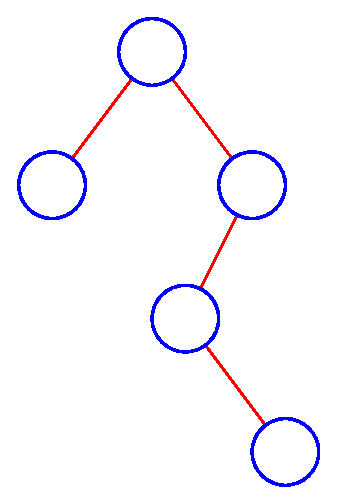
\includegraphics[height=4cm]{img/binTree}
   \caption{Binary tree}
 \label{fig:bintree}
 \end{subfigure}
~
 \begin{subfigure}[b]{0.3\textwidth}
   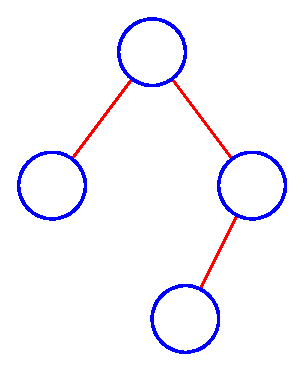
\includegraphics[height=4cm]{img/balanceTree}
   \caption{Balanced binary tree.}
   \label{fig:balancetree}
 \end{subfigure}
~
 \begin{subfigure}[b]{0.3\textwidth}
   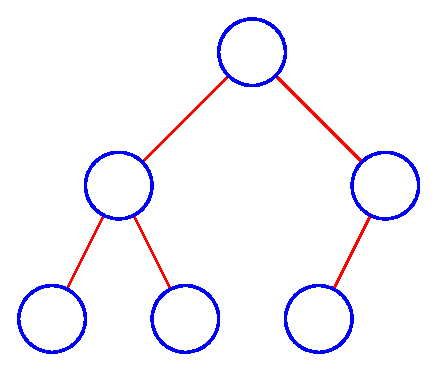
\includegraphics[height=4cm]{img/completeTree}
   \caption{Complete binary tree.}
   \label{fig:completetree}
 \end{subfigure}
  \caption{Properties of binary trees.}
  \label{fig:tree}
\end{figure}

A \emph{heap} is a data structure.
More specifically is a special kind of \emph{binary tree}, that is \emph{balanced} and \emph{complete}.
In addition, a heap has the following properties:
\begin{enumerate}
 \item The node at the root is \emph{greater} than all the other nodes in the tree\footnote{This is actually a \emph{max heap}. You can define analogously a \emph{min heap}, where the node at the root is \emph{smaller} than all the other nodes and so on.}.
 \item The previous property is also true for all the subtrees in the heap.
\end{enumerate}

Since we are comparing nodes, in a heap the nodes contain numeric values. The Figure~\ref{fig:heap} shows an example of a heap.

\begin{figure}[htb]
  \centering
  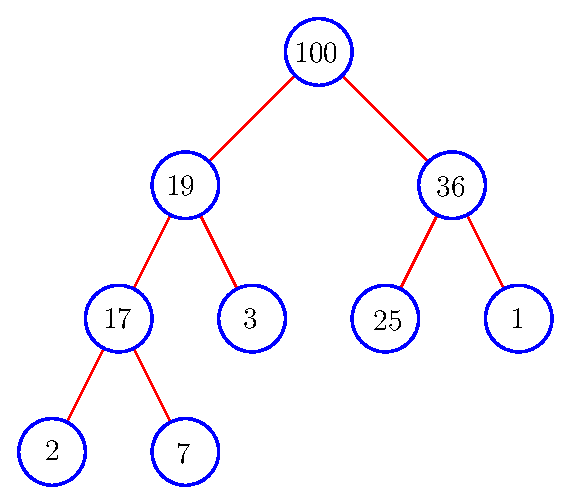
\includegraphics[width=0.45\textwidth]{img/heapTree}
  \caption{A heap represented as a tree}
  \label{fig:heap}
\end{figure}

\subsubsection{Heap implementation}

Thanks to the fact of being a complete and balanced binary tree it's possible to represent a heap using an array.

In a complete and balanced binary tree, we can define an order first per level and second inside each level from left to right.
Then we can use this order to store the values of all the nodes in a linear fashion (array) and think of them as if they were on the complete and balanced binary tree using the narural order of the array.

In order to do that we will need to define operations that enable us to locate a given node on the tree by only using his indices of the array.
The following functions works for that purpose:

\begin{align*}
P(i) & = \dfrac{(i - 1)}{2} \\
L_c(i) & = 2 \cdot i + 1 \\
R_c(i) & = 2 \cdot i + 2
\end{align*}

Where $P(i)$ returns the index of the parent, for the node whose index is $i$.
And $L_c$ and $R_c$ return the index of the left(right) child of the node whose index is $i$.

The Figure~\ref{fig:heaptree} shows the same heap of Figure~\ref{fig:heap} and Figure~\ref{fig:heaparray} shows his representation as an array.

\begin{figure}[htp]
\centering
 \begin{subfigure}[b]{0.3\textwidth}
   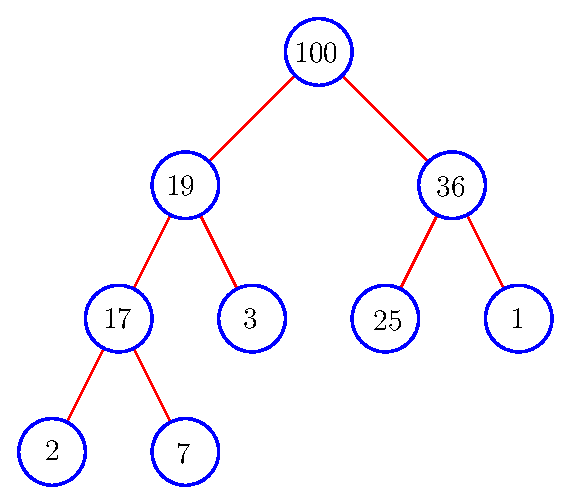
\includegraphics[width=\textwidth]{img/heapTree}
   \caption{Tree}
 \label{fig:heaptree}
 \end{subfigure}
~~
 \begin{subfigure}[b]{0.5\textwidth}
   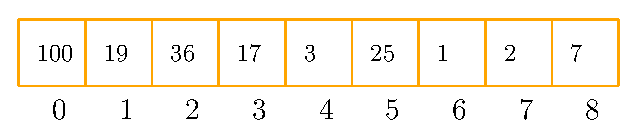
\includegraphics[width=\textwidth]{img/heapArray}
   \caption{Array.}
   \label{fig:heaparray}
 \end{subfigure}
\caption{Equivalent representations for a heap.}
\label{fig:heapRep} 
\end{figure}

Given an array of numbers that represents a heap we are interested in the following two operations\footnote{These are not the only operations defined for a heap, but rather the only ones we need to implement heapsort in the last section}:

\begin{description}
 \item[heapify] Given an array of elements we can compare (numbers), this operation will reorder the array, so it represents a heap. This operation in a well done implementation takes $O(n \cdot \lg n)$ and uses $O(1)$ extra memory.
 \item[sift down] If we \emph{change} the value of a given node of a heap, --and hence the heap property is ruined--. This operation will recompose the tree to be a valid heap again. This operation in a well done implementation takes $O(\lg n)$ for a heap with $n$ elements.
\end{description}

First, we well explaing how to perform the \emph{sift down} operation.
This operation is also named by some authors as \emph{percolate} down.
Since each subtree of a heap it's also a heap, we can assume without lossing generality that the node we just changed is the root.

\begin{algorithm}[H]
\caption{Sift down}
\label{alg:siftdown}
\begin{algorithmic}[1] % El número le dice al entorno desde que número empezar a contar. Si le pones 0 omite los números
\Require $H = \{ h_0, h_1, \ldots, h_{n-1} \} $, $h_b$ and $h_e$ \Comment{A heap $H$, the subheap $(h_b, h_e)$ whose root changed}
\Ensure $H$ as a valid heap
\Procedure{SiftDown}{$H$, $h_b$, $h_e$} \Comment{$b$ stands for \emph{begin} and $e$ for \emph{end}}

\EndProcedure
\end{algorithmic}
\end{algorithm}

\subsubsection{Sorting using a heap}
